% !TeX root = ../thuthesis-example.tex

\chapter{相关工作综述}

\section{引言}

本章对网络流量异常检测领域的相关工作进行综述。首先介绍校园网网络流量的特点,


异常检测是一个重要的领域,自1980年以来,国内外已经有无数学者在这方面做研究。分类、统计、信息理论和聚类。

\citet{ahmed2016survey}将异常检测技术分为分类、统计、信息理论和聚类四类。


本章还讨论了用于网络入侵检测的数据集的研究挑战。



\section{网络流量异常的定义和分类}
Hawkins(1980)给出了异常的本质性的定义\cite{hawkins1980identification}:异常是在数据集中与众不同的数据,使人怀疑这些数据并非随机偏差,而是产生于完全不同的机制。例如在道路交通领域,某条道路的车流量突然增多甚至堵塞或者突然减少,此时车流量数据就是一个异常。因此网络行为的异常就是指那些偏离了正常的、标准的或预期的行为。为了检测网络异常,网络所有者必须有一个预期或正常行为的概念,我们称其为基线。要检测网络行为的异常,就需要持续监控网络中的意外趋势或事件,那些可能改变网络流量特征或者监控指标的恶意行为。


因此我们只关注引起网络流量特征变化的恶意行为,而对于系统权限提升,缓冲区溢出等黑客攻击手段不做研究。
网络异常根据

网络流量异常具体有哪些类别,学术界没有统一的意见。本文中关注的网络流量异常按照产生意图分为恶意和非恶意两类,其中恶意行为主要有拒绝服务攻击,网络扫描,BGP劫持,网络蠕虫,僵尸网络等;非恶意行为主要有物理故障,突发事件等。接下来我们对这些异常分别进行介绍:

\begin{enumerate}
    \item 拒绝服务攻击:拒绝服务(DoS)攻击是一种网络攻击,恶意行为者的目的是通过中断计算机或其他设备的正常运作,使其目标用户无法使用该设备。DoS攻击的功能通常是通过构造大量请求淹没目标机器,直到正常的流量无法处理,导致额外用户的拒绝服务。分布式拒绝服务(DDoS)攻击是一种来自许多分布式来源的DoS攻击,如僵尸网络DDoS攻击。因其攻击成本低、攻击效果明显等特点,DDoS攻击仍然是互联网用户面临的最常见、影响较大的网络安全威胁之一。DoS攻击通常分为2类。(1)缓冲区溢出攻击:一种攻击类型,内存缓冲区溢出会导致机器消耗所有可用的硬盘空间、内存或CPU时间。这种形式的利用通常会导致行为迟缓、系统崩溃或其他有害的服务器行为,导致拒绝服务。(2)洪范攻击:通过用大量的数据包使目标服务器饱和,恶意行为者能够使服务器容量过饱和,导致拒绝服务。为了使大多数DoS泛滥攻击成功,恶意行为者必须拥有比目标更多的可用带宽。

    \item 网络扫描。网络扫描黑客在进行网络攻击之前,首先要进行网络扫描,从中寻找可以攻击的目标。具体来说,黑客需要确定网络中哪些主机是活动的,活动主机上运行了哪些存在漏洞的服务等,从而决定下一步的攻击计划。网络扫描分为主机扫描和端口扫描两种。

    主机扫描主机扫描的目的是确定网络中存在哪些在线的主机或设备。
    端口扫描端口扫描的目的是确定活动主机上开放了哪些端口,运行了哪些网络服务。按照扫描方式来分,端口扫描分为垂直扫描和水平扫描。垂直扫描会扫描某个主机的所有端口,而水平扫描则扫描网络中所有主机的某个固定端口。

    \item BGP劫持。BGP劫持是指攻击者恶意地对互联网流量进行重新路由。攻击者通过谎称拥有一组IP地址(称为IP前缀)的所有权来实现这一目的,而实际上他们并不拥有、控制或路由。BGP劫持就像有人把高速公路上的所有标志都换掉,把汽车流量改道到错误的出口。
    
    \item 网络蠕虫。网络蠕虫不同于计算机病毒。与计算机病毒不同的是,计算机蠕虫不需要附在别的程序内,可能不用用户介入操作也能自我复制或运行。计算机蠕虫未必会直接破坏被感染的系统,却几乎都对网络有害。计算机蠕虫可能会执行垃圾代码以发动分布式拒绝服务攻击,令计算机的执行效率极大程度降低,从而影响计算机的正常使用;可能会损毁或修改目标计算机的文件;亦可能只是浪费带宽。(恶意的)计算机蠕虫可根据其目的分成2类:

    一种是面对大规模计算机使用网络发动拒绝服务的计算机蠕虫,虽说会绑架计算机,但用户可能还可以正常使用,只是会被占用一部分运算、连网能力。
    另一种是针对个人用户的以执行大量垃圾代码的计算机蠕虫。计算机蠕虫多不具有跨平台性,但是在其他平台下,可能会出现其平台特有的非跨平台性的平台版本。第一个被广泛注意的计算机蠕虫名为:“莫里斯蠕虫”,由罗伯特·泰潘·莫里斯编写,于1988年11月2日释出第一个版本。这个计算机蠕虫间接和直接地造成了近1亿美元的损失。这个计算机蠕虫释出之后,引起了各界对计算机蠕虫的广泛关注。

    \item 僵尸网络。僵尸网络(简称 "机器人网络")是指由感染了恶意软件的计算机组成的网络,这些计算机由单一攻击方控制,即所谓的 "僵尸继承者"。在 "机器人携带者 "控制下的每一台机器都被称为 "机器人"。攻击方可以从一个中心点,指挥其僵尸网络上的每一台计算机同时进行协调的犯罪行动。僵尸网络的规模(许多僵尸网络由数百万个僵尸组成)使攻击者能够进行大规模的行动,这在以前的恶意软件中是不可能的。由于僵尸网络一直处于远程攻击者的控制之下,受感染的机器可以接收更新,并在飞行中改变其行为。因此,僵尸牧民往往能够在黑市上租用其僵尸网络部分的访问权,以获取大量经济利益。
    
    \item 物理故障是指路由器故障,链路破坏,断电等不可预测的突发事件。该类异常以两种方式影响着网络链路的流量。
    
    \item 突发事件。突发事件往往是正常的网络操作。
\end{enumerate}

% ddos,流氓推广,网络蠕虫,僵尸网络



% 异常检测所关注的异常是指那些造成网络流量特征改变的恶意行为。换句话说,如SQL注入,计算机病毒,系统权限提升,缓冲区溢出之类的恶意行为并不在异常检测的考虑范围内。异常检测所关注的网络异常大致分为如下几类:
% (1)
% 物理故障物理故障是指路由器故障,链路破坏,断电等不可预测的突发事件。该类异常以两种方式影响着网络链路的流量。

% 第一种是使直接相连的那些链路上的流量完全消失。
% 第二种是通过路由协议改变互联网中路由表,从而间接地改变其他链路的流量。
% (2)

% (3)
% BGP前缀劫持BGP前缀劫持是指黑客利用BGP协议(Broder Gateway Protocol)和路由转发算法的设计缺陷,恶意修改互联网路由表的内容,从而达到修改和控制数据包转发路径的目的W。BGP前缀劫持可能影响互联网上的每一个路由器,使得某一段IP地址范围成为一个“黑洞”,危害极其严重。

% (4)
% 基于协议或设备缺陷的攻击该类异常是指恶意用户利用网络协议或路由系统的设计漏洞而发动的攻击。属于该类异常的攻击有生成树(Spanning Tree)攻击,MAC表洪流,ARP(Address Resolution Protocol)攻击,VTP(VLAN Trunkong Protocol)攻击等[5]。

% (5)
% 拒绝服务攻击拒绝服务攻击是指黑客恶意破坏网络服务,降低网络的性能和可用性,使得受害主机无法正常地处理和回复客户请求的一种攻击行为。

% 美国计算机应急响应小组(US-CERT)给出了拒绝服务攻击的典型症状:网速极度缓慢,无法访问给定网站,无法访问任何网站,垃圾邮件数量激增,网络连接异常断开,服务器频繁掉线等。

% 按照攻击规模来分,拒绝服务攻击可以分为两大类,即拒绝服务攻击(DoS)和分布式拒绝服务攻击(DDoS)。

% 按照攻击方法来分,拒绝服务攻击可以分为剧毒包(Killer Packet)型攻击和风暴(FloodType)型攻击[6,7]。

% 剧毒包型剧毒包型攻击是指黑客利用网络协议,服务和系统的漏洞,只发送少量的数据包就可以达到拒绝服务的目的。
% 风暴型风暴型攻击并不依赖于系统和协议的漏洞,而是向受害网络或主机暴力地发送大量的数据包,从而达到阻塞网络,耗尽系统资源的目的。
% (6)
% 蠕虫蠕虫本质上是一段传播性极强的恶意代码,通过扫描主机系统和应用软件的漏洞或者通过发送钓鱼邮件,将自己复制到目标主机上并获得控制权限,随后安装木马或后门,并以目标主机为基地重复上述扫描过程。蠕虫的传播速度呈几何级数增长,能够在很短的时间感染整个互联网,危害极大。典型的懦虫有Klez懦虫、MyDoom懦虫、Sasser懦虫、SQL Slammer懦虫和Blaster懦虫等。

% (7)
% 非恶意行为该类异常并非是源于黑客攻击或恶意代码,而是源于一些正常的网络应用或操作。然而,这些正常的行为往往会间接地导致网络流量的变化或性能的下降。属于该类异常的行为有:

% Alpha Flow是指那些在单点到单点之间产生大量流量的应用,如高清视频下载,带宽测量实验,传送大量文件等。
% 瞬时拥塞(Flash Crowds) 瞬时拥塞是指用户数目在短时间内急剧增长,生成了大量流量,从而导致链路拥塞的现象。比如某个网站发布了最新版本的Linux,大量用户的下载行为就会导致瞬时拥塞。再如某个网站发布了一则关于政治人物的丑闻,大量用户浏览网页的行为同样会导致瞬时拥塞。瞬时拥塞与分布式拒绝服务攻击的区别在于瞬时拥塞属于用户正常行为,而分布式拒绝服务攻击则属于黑客的恶意攻击行为。
% 入口切换(Ingress Shift) 为了提高链路和网站的性能和可靠性,Internet内容提供商(ICP)往往采用多路径连接(Multi-Homing)的策略,即将自己的网络接入多个Internet服务提供商(ISP)的多个入口链路上。如此一来,一方面增加了带宽,利于部署负载均衡;一方面大大降低了Internet接入中断的风险。入口切换就是指Internet内容提供商基于某种策略,将流量从一个入口链路切换到另一个入口链路的行为。了解这类异常有助于网络管理员进行网络诊断,负载均衡,流量工程,链路规划等,因而这种本无恶意的行为也成为了异常检测所关注的对象。



\section{网络流量异常检测算法}
% 目前,学术界和工业界已经提出了一系列 KPI 异常检测算法。这些算法可以概括地分成基于窗口的异常检测算法,例如奇异谱变换 (singular spectrum transform) ;基于近似性的异常检测算法 ;基于预测的异常检测算法,例如 Holt-Winters 方法、时序分解方法、线性回归方法、支持向量回归等 ;基于隐式马尔科夫模型的异常检测算法 ;基于分段的异常检测算法 ;基于机器学(集成学习的异常检测算法等类别。

% \subsection{基于时间序列的异常检测}
% 时间序列是将某种统计指标的数值,按时间先后顺序排序所形成的数列。时间序列的预测就是通过分析时间序列,根据时间序列所反映出来的发展过程、方向和趋势,进行类推或延伸,预测下一段时间或以后若干年内可能达到的水平。时间序列的异常检测就是通过历史的数据分析,查看当前的数据是否发生了明显偏离了正常的情况。主要的时间序列模型有移动平均、指数平均等等。
% IMC’2015[3]通过有监督的机器学习算法来解决手动和迭代的调整检测器参数和阈值的难题。多年来,人们提出了数十种异常检测器,用于密切监控设备性能及发现异常。但是部署它们是一个巨大的挑战,需要人工手动和迭代的调整检测器参数和阈值。

% 该文章通过对多个检测器中的性能数据提取异常特征;然后用特征和标签训练随机森林分类器,自动选择适当的参数和阈值。有以下局限性:
% 1.有监督学习需要带标签的数据;
% 2.这种算法受限于训练集中的异常,也就是无法判别未来出现的新的异常;
% 因此,WWW’2018[4]提出了无监督的机器学习算法,即针对周期性KPI数据,使用基于VAE(变分自动编码器)的异常检测算法。

% \subsection{基于日志的异常检测}
% 系统产生的日志是非结构化文本,并且有信息量巨大、类型繁多等特点,这就为分析日志带来了许多困难。主要有以下几点挑战: 

% 1.系统越来越多地由多个组件,尤其是分布式组件构成,使用单个日志文件监视系统变得不可能。交叉异构的日志文件很难分析,特别是当时间戳不同步甚至不存在的时候。
% 2.最大化日志系统的信息量的同时最小化检测成本。
% 3.单纯的统计模型并不能提供可行性建议。例如,可以用机器学习模型来发现负载中的异常,CPU利用率过高,但是无法解释应该怎么处理。
% CCS’2017[5] 提出了一种基于深度学习的日志异常检测系统——DeepLog。DeepLog通过以下三步异常检测来综合判断系统异常.
% 1.执行路径异常检测。将异常检测问题转换成一个log key的多分类问题,使用LSTM对日志的log key序列建模, 自动从正常的日志数据中学习正常的模式并且由此来判断系统异常。同时,LSTM可以增量式地调整模型参数,以便适应随着时间推移而出现的新日志文件。
% 2.参数和性能异常检测。有时候系统虽然是按照正常操作步骤执行的,但是记录的日志中的参数是不正常的,比如延迟比正常要大,这种情况也属于异常。
% 3.工作流异常检测。虽然工作流模型在异常检测的有效性上不如LSTM模型,但是工作流模型可以可视化地帮助运维工程师在发现异常后找出异常的原因。
% 其中长短期记忆(Long short-term memory, LSTM)是一种特殊的RNN,主要是为了解决长序列训练过程中的梯度消失和梯度爆炸问题。相比普通的RNN,LSTM能够在更长的序列中有更好的表现。

本节将介绍在异常检测领域主流的一些算法,根据所依赖的技术原理的不同,将这些算法分为了基于统计、基于分类、基于聚类、基于信息论、基于深度学习的异常检测算法。

\subsection{基于分类的异常检测算法}

基于分类的技术依赖于专家对网络攻击特征的广泛了解。当网络专家向检测系统提供详细的特征时,具有已知模式的攻击一经发起就能被检测出来。这完全依赖于攻击的签名,作为一个系统,只有当网络专家较早地提供了攻击的签名,它才能够检测出攻击。这说明一个只能够检测到它所知道的系统很容易受到新的攻击,而新的攻击会不断出现不同的版本,并且更加隐蔽地发起。即使创建了新的攻击的签名并将其纳入系统中,最初的损失也是不可替代的,而且修复程序非常昂贵。

基于分类的方法依赖于建立知识库的正常流量活动特征,并将偏离基线特征的活动视为异常活动。其优势在于它们能够检测到完全新颖的攻击,假设它们表现出大量的偏离正常配置文件的情况。此外,由于知识库中未包含的正常流量被认为是攻击,因此会有无意中的误报。因此,异常检测技术需要进行训练,以建立正常的活动配置文件,这很耗时,而且还取决于是否有完全正常的流量数据集。在实践中,获得无攻击的流量实例是非常罕见且昂贵的。此外,在当今׳s动态和不断变化的网络环境中,保持正常配置文件的更新是非常困难的。在现有的大量基于分类的网络异常检测技术中,我们主要讨论以下四种技术。

\citet{2002AEskin} 引入无监督SVM的概念来检测异常事件。常规的SVM的原理是推导出一个超平面,使得正类样本和负类样本之间的分离余量最大化,将特征空间中的两类数据进行分离。标准的SVM算法是一种监督学习方法,需要标记数据来创建分类规则。而该算法经过改进SVM,试图将整个训练数据集从原点分离出来,找到一个以最大余量将数据实例与原点分离的超平面,

\citet{Hu2003Robust} 提出了一种忽略噪声数据的异常检测方法,该方法使用Robust SVM(RSVM)来开发。标准的SVM有一个主要假设,即所有的训练样本数据都是独立且相同分布的(i.i.d)。但是在实际场景中,训练数据往往包含噪声,这就会导致标准SVM会学习出一个高度非线性的决策边界,从而导致通用性较差。基于此,RSVM以类中心的形式加入了平均化技术,使得决策面更加平滑。此外,RSVM另一个优点是能大大降低支持向量的数量,从而减少运行时间,提高效率。

% TODO
\citet{kruegel2003bayesian} 假设异常检测系统包含许多模型,用于分析一个事件的不同特征,指出了在这种系统下异常检测技术造成高误报率的两个主要原因。一是异常检测系统通过将多个概率模型的输出进行汇总,而每个模型往往只给出一个事件的常态/异常的得分或概率,从而导致高误报率;二是异常检测系统无法处理那些不正常但合法的行为,如CPU利用率、内存使用率突然增高等。基于贝叶斯网络的概念,\citet{kruegel2003bayesian}提出了一种解决上述问题的方法。对于一个输入事件的有序流($\symbf{S}=e_1,e_2,e_3...$),异常检测系统决策每个事件是正常还是异常。该决策基于k个模型($\symbf{M}=m_1,m_2,...,m_k$)的输出($o_i|i=1,2,...,k$)和可能的附加信息($\symbf{I}$)。应用贝叶斯网络来识别异常事件,引入根节点,根节点代表一个具有两种状态的变量。一个子节点用于捕捉模型׳的输出,子节点与根节点相连,预计当输入异常或正常时,输出事件会有所不同。贝叶斯网络最近的应用可以在电信网络中找到(Deljac等,2015)。
贝叶斯网络是对包含不确定性的领域进行建模的一种有效方法。一个离散的随机变量用一个有向无环图(DAG)表示,其中每个节点反映了随机变量的状态,并包含一个条件概率表(CPT)。CPT的任务是提供一个节点处于特定状态的概率。在贝叶斯网络中,节点之间存在着父子关系,这表明子节点所代表的变量依赖于父节点所代表的变量。由于这种网络可以用于事件分类方案,因此也适用于网络异常检测。


神经网络已经被应用于各个应用领域,如图像和语音处理,但其对计算量的要求很高。神经网络对数据进行分类的优势也可被用于网络异常检测。在网络异常检测领域,神经网络通常会和其他技术进行结合,如统计方法。2020outlier 提出了一个多层的前馈神经网络,该神经网络可以用来进行异常值的检测。具体来说,Replicator Neural Networks是一个多层前馈的神经网络 (multi-layer feed-forward neural networks),在输入层和输出层之间放置了三个隐藏层。它的目标是通过训练在输出层以最小的误差重现输入数据模式。由于该模型中间隐藏层节点的个数少于输入输出层节点的个数,这样就起到了压缩数据和恢复数据的作用。
RNN的示意图如图~\ref{fig:rnn}所示。

\begin{figure}
    \centering
    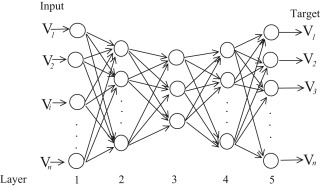
\includegraphics[width=0.6\linewidth]{RNN.jpg}
    \caption{Replicator Neural Networks示意图}
    \label{fig:rnn}
  \end{figure}
% 这类方法通常是将异常检测看成是数据不平衡下的分类问题。常用分类算法有朴素贝叶斯、逻辑回归、支持向量机等。
% 以支持向量机(SVM)为例,SVM在集成学习和神经网络之类的算法没有表现出优越性能前,基本占据了分类模型的统治地位。
% 目前由于互联网数据规模的急剧膨胀,SVM无法很好的处理海量样本,热度有所下降,但是仍然是一个常用的机器学习算法。
% 在异常检测领域中,当异常值远远少于正常值时,可以用One-Class SVM。当异常值较多即正负样本均衡时,适用于普通的二分类SVM。可以根据样本情况灵活调整。
% One-Class SVM的输入为不包含异常值的“干净”数据,试图求得高维空间的一个超球面,以最小的半径将训练集中的数据包起来。新来的待测数据映射到高维空间后,如果落在这个超球面之外,则认为它是一个异常值。

\citet{2001HIDE} 提出了一种神经网络与统计模型相结合的分层入侵检测系统。将神经网络分类器的输出表示为一个连续变量($t$),其中-1表示有绝对把握的入侵,1表示没有攻击。此外,自组织地图(SOM)被用于网络异常检测。Ramadas等(2003)提出,利用SOM,可以对网络流量进行实时分类。SOM依赖于这样一个假设,即网络攻击可以由不同的神经元组来描述,这些神经元组与其他神经元组相比,在输出神经元图上覆盖更大的区域。\citet{5592568} 开发了一个由反向传播算法训练的前馈神经网络,利用给定的数据集与计算机网络在正常和异常行为期间的相关信息来检测异常。

\subsection{基于统计的异常检测算法}

早期的异常检测方法往往基于统计与概率模型,也就是假设-检验的方法。首先对数据的分布做出假设,然后找出假设下所定义的“异常”,因此往往使用极值分析或假设检验。
比如对最简单的一维数据假设服从正态分布,然后将距离均值某个范围以外的点当做异常点。推广到高维后,假设各个维度相互独立。这类方法的好处速度一般比较快,但是因为存在很强的“假设”,效果不一定很好。

% \citet{Nong2010An} 基于卡方检验的距离测量方法,将卡方检验的理论应用于异常检测。根据此技术,首先需要建立一个正常事件的基线,该方法的
入侵检测技术也是利用统计理论发展起来的;例如,Ye和Chen(2001年)在异常检测中使用了成熟的chi-square理论。根据这种技术,建立了一个信息系统中正常事件的档案。这种方法的基本思想是既要检测出与正常事件有较大偏差的异常事件,又要检测出入侵事件。基于chi-square检验统计量的距离测量方法被开发为
\begin{equation}
    \chi^2 = \sum_{i=1}^n \frac{(X_i - E_i)^2}{E_i}
\end{equation}

其中$X_i$为第$i$个变量的观测值,$E_i$为第$i$个变量的期望值,$n$为变量的数量。

当一个变量的观测值接近预期时,$\chi^2$的值就会很低。根据$3\sigma$定律,当观测值的$\chi^2$大于$\bar{X^2}+3S_X^2$时,该值被视为异常。

\citet{Christopher2002Service} 提出了一种用于检测异常网络流量的统计处理单元,更具体地说,是为了检测R2L和U2R等罕见的攻击。开发了一种度量方法,使系统能够自动搜索不同服务请求的相同特征。根据以下三个主要特征计算出请求的异常得分。
请求的类型;
请求的长度;以及
有效载荷分布。
网络管理员定义了一个阈值,以便对异常请求发出警报。异常得分的计算方法如式(5),其中有效负载分布的权重大于其他属性。(5)
基于统计学理论的原理,我们开发了不同类型的技术来检测异常,接下来将讨论。

在时间序列异常检测领域,最常见的基于统计的算法为ARIMA,即差分自回归移动平均模型[8]。我们将流量信号分解为两部分,一是遵循一定规律、可预测的正常变化,二是由突发性变化组成、不可预测的异常情况。ARIMA分析和建模用于网络流量预测,能够检测和识别流量异常或异常值。


\subsection{基于信息论的异常检测算法}

信息理论的测量方法可以用来建立一个适当的异常检测模型。在Lee和Xiang(2001)的一篇论文中,使用了几种度量方法,如熵、条件熵、相对熵、信息增益和信息成本来解释数据集的特征。我们对这些度量方法的定义如下。

熵是信息论的一个基本概念,它衡量一个数据项集合的不确定性。对于一个数据集D,其中每个数据项都属于一个类(x ),D相对于分类的熵定义为: 1.
(13)
其中P(x)为x在D中的概率。


条件熵是指D的熵,给定Y是概率分布()的熵,为
(14)
其中P(x,y)是x和y的联合概率和x给定y的条件概率。


相对熵是指定义在相同的两个概率分布p(x)和q(x)之间的熵,具体为
(15)

相对条件熵是指定义在同一和上的两个概率分布(和)之间的熵。
(16)

信息增益是对数据集D中某一属性或特征A的信息增益的衡量,是
(17)
其中,值A为A的可能值集,Dv为D的子集,其中A的值为v。


Ambusaidi等人(2014)中提出了一种基于非线性相关系数(NCC)的相似性测量方法,以提取网络流量之间的线性和非线性相关性。提取的相关信息用于检测恶意网络行为。Pearson׳s相关系数是一种基本的线性相关方法,用于找出两个变量之间的依赖关系(Ahmed等,2015c),然而,在一些数据集中,不同变量之间存在非线性相关,如网络流量中。NCC由Wang等(2005)定义,如式(18),其中和为变量X和Y的修正熵。

给定一组m个正常训练数据实例,首先计算NCC。对于任何传入实例,传入实例与正常实例之间的NCC记录为 。对于用户定义的阈值σ,其范围在0和1之间,如果NCC的差异大于σ,则认为一个传入流量实例是异常的(19)。


在Tan等(2014a)中,针对DoS攻击检测,提出了一个利用多元相关分析(MCA)的系统,通过提取网络流量特征之间的几何相关性,来实现网络流量的精确特征分析。检测过程主要包含三个步骤,如图6所示。在步骤1中,在一个明确的时间区间内生成基本特征。第2步包含多元相关分析,应用 "三角区域图生成 "模块,提取第一步得出的每个流量实例中两个不同特征之间的相关性。第三步是基于训练和测试阶段的决策。


基于这些知识,可以建立适当的异常检测模型。有监督的异常检测技术需要先有一个训练数据集,再有一个测试数据来评估模型的性能。在这种情况下,首先,使用信息理论措施来确定模型是否适合测试新数据集。Noble和Cook(2003)在基准DARPA和UNM审计数据集上进行了实验,以证明信息理论措施的效用,并得出结论,它们可以用来创建高效的异常检测模型,也可以用来解释它们的性能

Tan等人(2014a)中的多变量相关分析方法的概念被纳入到网络流量实例的表征中,并将其转换为相应的图像。这些图像被用于DoS攻击检测,基于一个广泛使用的异构度量,即地球移动者距离(Earth Mover׳s Distance,EMD)(Rubner等,1998)。EMD考虑了跨区域匹配,比其他一些著名的异同度测量方法更准确地评估了分布之间的异同度。

\subsection{基于聚类的异常检测算法}

聚类指的是无监督学习算法,它不需要预先标记数据来提取相似数据实例的分组规则(Jain等,1999)。虽然有不同类型的聚类技术,但我们讨论常规聚类和共聚类对网络异常检测的有用性。常规聚类和共聚类的区别在于行和列的处理。常规聚类技术如k-means(Ahmed和Naser,2013)考虑数据集的行进行聚类,而共聚类则同时考虑数据集的行和列来产生聚类(Ahmed等人,2015d)。

下面简单讨论一下使用聚类检测异常时总是要做的三个关键假设。
假设1:由于我们只能创建正常数据的聚类,因此,后续任何与现有正常数据聚类不相适应的新数据都被认为是异常数据;例如,由于基于密度的聚类算法不包括聚类内的噪声(Ester等人,1996),噪声被认为是异常数据。

假设2:当一个簇同时包含正常数据和异常数据时,已经发现正常数据靠近最近的簇中心点,但异常数据远离中心点(Ahmed和Naser,2013)。在这种假设下,异常事件使用距离得分来检测。

假设3:在一个具有不同大小的聚类中,较小和较稀疏的聚类可以被认为是异常的,较厚的聚类是正常的。属于大小和/或密度低于阈值的聚类的实例被认为是异常的。


Münz等人(2007)对异常数据采用的方法非常直接。他们使用k-means聚类来生成正常和异常聚类。一旦实现聚类,就使用以下假设进行分析。

如果一个实例比异常簇中心点更接近正常,则该实例被列为正常,反之亦然。


如果实例与中心点之间的距离大于预定义的阈值(dmax),则该实例被视为异常;以及


如果一个实例比正常聚类中心点更接近异常聚类中心点,或者它与正常聚类中心点的距离大于预定义的阈值,则被视为异常。


Petrovic等(2006)提出了一种基于聚类评价技术组合的聚类标签策略。将Davies-Bouldin聚类评价指数和聚类中心直径的比较结合起来,以充分应对攻击向量的特性。他们考虑了相应聚类的紧凑性和它们之间的分离度,以及区分分析网络中 "正常 "和 "异常 "行为的主要参数。然而,他们并没有解释他们的k-means聚类使用k=2的原因。根据他们的方法,攻击向量通常非常相似,如果不是完全相同的话;例如,在大规模攻击的情况下,相应的聚类是非常紧凑的,这种聚类的Davies-Bouldin指数要么是0(当非攻击聚类是空的时候),要么是非常接近0。考虑到攻击向量之间的预期相似性,因为攻击聚类的中心点的直径预期比非攻击聚类的直径小,他们可以区分正常和异常的聚类。

Portnoy等(2001)提出了基于宽度的聚类来对数据实例进行分类。宽度是恒定的,对所有聚类都保持不变。一旦进行聚类,基于正常实例在整个数据集中占压倒性比例的假设,N\%的聚类是正常的,其余是异常的。利用这一假设,Leung和Leckie(2005)提出了一种基于密度和网格的聚类算法,该算法适用于无监督的异常检测。

Syarif等人(2012)研究了各种聚类算法应用于异常检测时的性能。他们使用了五种不同的方法,即k-means、改进的k-means、k-medoids、期望值最大化(EM)聚类和基于距离的异常检测算法。表3展示了用于网络异常检测的聚类算法的性能评价。



聚类算法通常是基于距离/密度发现异常点。基于距离/密度的异常点检测方法的关键步骤在于给每个数据点都分配一个离散度,其主要思想是:
针对给定的数据集,对其中的任意一个数据点,如果在其局部邻域内的点都很密集,那么认为此数据点为正常数据点,而异常点则是距离正常数据点最近邻的点都比较远的数据点。通常有阈值进行界定距离的远近。
异常检测领域下常用的聚类算法有k-means、LOF、孤立森林、高斯混合模型[20]等。

\subsection{基于深度学习的异常检测算法}
随着深度学习的兴起,越来越多的学者尝试用深度学习算法来进行异常检测,尤其是针对时间序列数据,深度学习模型往往表现出惊人的效果。
常用的深度学习算法为变分编码器、神经网络[6][14]、生成对抗网络、LSTM[17]、RNN[3][4][10][12][13][15]等。以变分自动编码器(Variational Auto-Encoder)[5]为例,其利用自编码器的重构误差和局部误差,针对时间序列的异常检测的场景,达到了很好的效果。

\section{异常检测领域开源数据集介绍}
数据集主要由KDDCUP99, CICIDS等。网络流量异常检测领域最为经典的数据集当属KDD99,但是这个数据集年代过于久远,对于现在的网络环境早已不适用。 NSL-KDD是为了解决KDD'99数据集的一些固有问题而提出的数据集,这些问题在[1]中已经提到。虽然,这个新版本的KDD数据集仍然存在McHugh所讨论的一些问题,并且可能不能完美地代表现有的真实网络,但由于缺乏基于网络的IDS的公共数据集,我们相信它仍然可以作为一个有效的基准数据集来帮助研究人员比较不同的入侵检测方法。

此外,NSL-KDD训练集和测试集的记录数量是合理的。这一优势使得在完整的集合上运行实验是经济实惠的,而不需要随机选择一小部分。因此,不同研究工作的评价结果将具有一致性和可比性。

CICIDS2017数据集包含了良性的和最新的常见攻击,与真实的现实世界数据(PCAPs)相似。它还包括使用CICFlowMeter进行网络流量分析的结果,并根据时间戳、源和目的IP、源和目的端口、协议和攻击(CSV文件)对流量进行了标注。同时还提供了提取的特征定义。

生成真实的背景流量是我们构建这个数据集的首要任务。我们使用了我们提出的B-Profile系统(Sharafaldin,等人,2016)来对人类交互的抽象行为进行剖析,并生成自然的良性背景流量。对于这个数据集,我们基于HTTP、HTTPS、FTP、SSH和电子邮件协议建立了25个用户的抽象行为。

数据采集期从2017年7月3日(周一)上午9点开始,到2017年7月7日(周五)下午5点结束,共5天。其中周一为正常日,只包括良性流量。实施的攻击包括蛮力FTP、蛮力SSH、DoS、Heartbleed、Web攻击、渗透、僵尸网络和DDoS。它们在周二、周三、周四和周五的上午和下午都被执行过。

在我们最近的数据集评估框架中(Gharib等人,2016),我们确定了建立一个可靠的基准数据集所必需的11个标准。之前的IDS数据集都无法覆盖这11项标准的全部内容。在下文中,我们简要地概述了这些标准。

THU-IDS 清华校园网数据集,该数据集为真实流量,将于第三章进行介绍。

% https://www.unb.ca/cic/datasets/nsl.html
\section{异常检测算法对比}
对比
不同机器学习方法在NSL-KDD数据集上的效果,
\section{现有异常检测算法存在的问题}